\documentclass[a4 paper]{article}
\usepackage[inner=2.0cm,outer=2.0cm,top=2.5cm,bottom=2.5cm]{geometry}
\usepackage{setspace}
\usepackage[ruled]{algorithm2e}
\usepackage[rgb]{xcolor}
\usepackage{verbatim}
\usepackage{subcaption}
\usepackage{amsgen,amsmath,amstext,amsbsy,amsopn,tikz,amssymb,tkz-linknodes}
\usepackage{fancyhdr}
\usepackage[colorlinks=true, urlcolor=blue,  linkcolor=blue, citecolor=blue]{hyperref}
\usepackage[colorinlistoftodos]{todonotes}
\usepackage{rotating}
\usepackage{booktabs}
\newcommand{\ra}[1]{\renewcommand{\arraystretch}{#1}}

\usepackage{minted}


\renewcommand{\theFancyVerbLine}{
  \sffamily\textcolor[rgb]{0.5,0.5,0.5}{\scriptsize\arabic{FancyVerbLine}}}



\newtheorem{thm}{Theorem}[section]
\newtheorem{prop}[thm]{Proposition}
\newtheorem{lem}[thm]{Lemma}
\newtheorem{cor}[thm]{Corollary}
\newtheorem{defn}[thm]{Definition}
\newtheorem{rem}[thm]{Remark}
\numberwithin{equation}{section}

\newcommand{\homework}[6]{
   \pagestyle{myheadings}
   \thispagestyle{plain}
   \newpage
   \setcounter{page}{1}
   \noindent
   \begin{center}
   \framebox{
      \vbox{\vspace{2mm}
    \hbox to 6.28in { {\bf MATH 118:~Statistics and Probability \hfill {\small (#2)}} }
       \vspace{6mm}
       \hbox to 6.28in { {\Large \hfill #1  \hfill} }
       \vspace{6mm}
       \hbox to 6.28in { {\it Instructor: {\rm #3} \hfill Name: Ahmed Semih Özmekik{\rm #5} \hfill Student Id: 171044039 {\rm #6}} \hfill}
       \hbox to 6.28in { {\it Assistant: #4  \hfill #6}}
      \vspace{2mm}}
   }
   \end{center}
   \markboth{#5 -- #1}{#5 -- #1}
   \vspace*{4mm}
}

\newcommand{\problem}[2]{~\\\fbox{\textbf{Problem #1}}\hfill (#2 points)\newline\newline}
\newcommand{\subproblem}[1]{~\newline\textbf{(#1)}}
\newcommand{\D}{\mathcal{D}}
\newcommand{\Hy}{\mathcal{H}}
\newcommand{\VS}{\textrm{VS}}
\newcommand{\solution}{~\newline\textbf{\textit{(Solution)}} }

\newcommand{\bbF}{\mathbb{F}}
\newcommand{\bbX}{\mathbb{X}}
\newcommand{\bI}{\mathbf{I}}
\newcommand{\bX}{\mathbf{X}}
\newcommand{\bY}{\mathbf{Y}}
\newcommand{\bepsilon}{\boldsymbol{\epsilon}}
\newcommand{\balpha}{\boldsymbol{\alpha}}
\newcommand{\bbeta}{\boldsymbol{\beta}}
\newcommand{\0}{\mathbf{0}}


\begin{document}
\homework{Homework \#4}{Due: 22/06/20}{Dr. Zafeirakis Zafeirakopoulos}{Gizem S\"ung\"u}{}{}
\textbf{Course Policy}: Read all the instructions below carefully before you start working on the assignment, and before you make a submission.
\begin{itemize}
\item It is not a group homework. Do not share your answers to anyone in any circumstance. Any cheating means at least -100 for both sides. 
\item Do not take any information from Internet.
\item No late homework will be accepted. 
\item For any questions about the homework, send an email to gizemsungu@gtu.edu.tr.
\item Submit your homework (both your latex and pdf files in a zip file) into the course page of Moodle.
\item Save your latex, pdf and zip files as "Name\_Surname\_StudentId".\{tex, pdf, zip\}.
\item The answer which has only calculations without any formula and any explanation will get zero. 
\item The deadline of the homework is 22/06/20 23:55.
\item I strongly suggest you to write your homework on \LaTeX. However, hand-written paper is still accepted \textbf{IFF} your hand writing is \textbf{clear and understandable to read}, and the paper is well-organized. Otherwise, I cannot grade your homework.
\item You do not need to write your Student Id on the page above. I am checking your ID from the file name.
\end{itemize}

\problem{1:}{10+10+10+10+10+10+40 = 100}
\textbf{WARNING:} Please show your OWN work. Any cheating can be easily detected and will not be graded.
\newline
\newline
For the question, please follow the file called airplane\_crashes.txt while reading the text below.\\
\newline
In each year from 1993 to 2012, the number of airplane crashes in airline companies were counted. The data was collected from 14 different airline companies. The numbers of crashes for the airline companies are indicated in 14 columns following the year column. Assume that the number of crashes per airline company per year is a random variable having a Poisson($\lambda$) and that the number of crashes in different airline company or in different years are independent.\\
(Note: You should implement a code for your calculations for each following subproblem. You are free to use any programming languages (Python, R, C, C++, Java) and their related library.)

\subproblem{a} Give a table how many cases occur for all companies between 1993 and 2012 for each number of crashes (\# of Crashes).\\
Hint: When you check the file you will see: \# of Crashes = \{0, 1, 2, 3, 4\}.\\
\newpage
\begin{table}[htb!]
	\centering
	\begin{tabular}{c|c}
		\begin{tabular}[c]{@{}c@{}}\textbackslash{}\# of\\Crashes\end{tabular} & \begin{tabular}[c]{@{}c@{}}\textbackslash{}\# of cases\\in all company \\between the years\end{tabular}  \\ 
		\hline
		0                                                                      &                          144                                                                                \\
		1                                                                      &                             91                                                                             \\
		2                                                                      &                              32                                                                            \\
		3                                                          & 11 
		\\ 
		4                                                                      &                                                2                                                        
	\end{tabular}

\caption{Actual cases}
\label{tab1}
\end{table}

\subproblem{b} Estimate $\lambda$ from the given data. \\

This calculation was done with code, you can check below for calculation. $\lambda$ is 0.7.

\subproblem{c} Update Table \ref{tab1} in Table \ref{tab2} with Poisson predicted cases with the estimated $\lambda$.\\
\begin{table}[htb!]
	\centering
	\begin{tabular}{c|c|c}
		\begin{tabular}[c]{@{}c@{}}\textbackslash{}\# of\\Crashes\end{tabular} & \begin{tabular}[c]{@{}c@{}}\textbackslash{}\# of cases\\in all companies\\between the years\end{tabular} & \begin{tabular}[c]{@{}c@{}}Predicted \textbackslash{}\# of cases\\in all companies\\between the years\end{tabular}  \\ 
		\hline
		0                                                                      &                                                                                                 144         &                    139.04388506159466                                                                                                 \\
		1                                                                      &                                                                                                      91    &                     97.33071954311626                                                                                                \\
		2                                                                      &                                                                                                       32   &                     34.065751840090684                                                                                               \\
		3                                                                      &                                                                                                      11    &    7.948675429354493    
		\\
		4                                                                      &                                                                                                      2    &             1.3910182001370366                                                                                                     
	\end{tabular}
\caption{Actual vs. Predicted Cases}
\label{tab2}
\end{table}
\subproblem{d} Draw a barplot for the actual cases (Table \ref{tab2} in column 2) and the predicted cases (Table \ref{tab2} column 3) with respect to \# of crashes. You should put the figure.\\

\begin{figure}[h!]
    \centering
    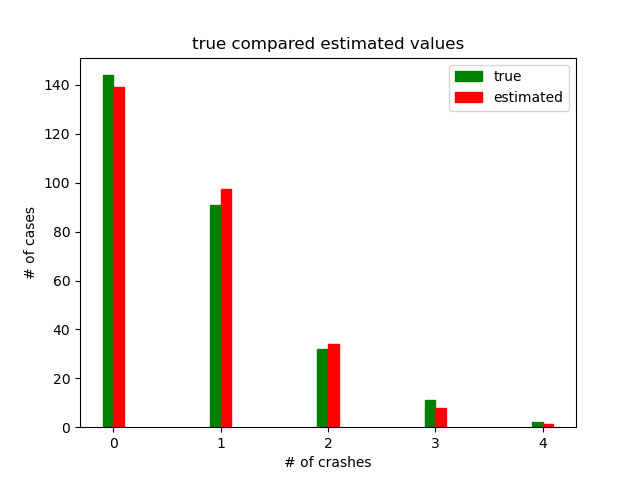
\includegraphics[scale=0.6]{plot.png}
    \caption{Actual vs. Predicted Cases}
    \label{fig:barplot}
\end{figure}

\subproblem{e} According to the barplot in (c), does the poisson distribution fit the data well? Compare the values of the actual cases and the values of the poisson predicted cases, and write your opinions about performance of the distribution.\\

Difference list: [ 4.95611494, -6.33071954, -2.06575184,  3.05132457,  0.6089818 ]
They are very close, and we can say the distribution fit the data well.

\subproblem{f} According to your estimations above, write your opinions considering your barplot and Table \ref{tab2}. Do you think that airplane transportation is dangerous for us? Whether yes or no, explain your reason.

In my opinion, airplane transportation seems not dangerous, according to the the poisson distribution = 0.503.


\subproblem{g} Paste your code that you implemented for the subproblems above. Do not forget to write comments on your code.\\
Example:\\
\begin{itemize}
	\item The common code block for all subproblems\\
	\begin{minted}[mathescape,
               linenos,
               numbersep=5pt,
               gobble=2,
               frame=lines,
               framesep=2mm]{csharp}
               
    import math
    import numpy as np
    import matplotlib.pyplot as plt

    CRASH = 5

    def input():
        file = open("airplane_crashes.txt", "r")
        X = []
        for line in file:
            stripped_line = line.strip()
            line_list = stripped_line.split()
            X.append(line_list)
        file.close()
        return X
    def num_of_case(X, crash_num):
        count = 0
        for line in X:
            count += line[1:].count(str(crash_num))
        return count
        
    X = input()

    company_count = len(X[0]) - 2
    year_count = len(X)

    real_table = print_table_a(X)

    # find lambda
    mean = find_lambda(X, company_count, year_count)
    print(mean)

    # find estimations
    estimated_table = estimate([i for i in range(len(real_table))], mean, company_count, year_count)
    print(estimated_table)

    # plot
    barplot(real_table, estimated_table)

    # difference
    print(np.array(real_table) - np.array(estimated_table))
  
\end{minted}
	\item The code block for (a)\\
	\begin{minted}[mathescape,
               linenos,
               numbersep=5pt,
               gobble=2,
               frame=lines,
               framesep=2mm]{csharp}
               
    def print_table_a(X):
        table_a = []
            for i in range(0, CRASH):
                table_a.append(num_of_case(X, i))
        print("{}\t{}".format(i, table_a[i]))
        return table_a
  
\end{minted}
	
	
	\item The code block for (b)\\
	\begin{minted}[mathescape,
               linenos,
               numbersep=5pt,
               gobble=2,
               frame=lines,
               framesep=2mm]{csharp}
               
    def find_lambda(X, cc, yc):
        total_case = 0
            for i in range(0, CRASH):
                total_case += i * num_of_case(X, i)
        return total_case / (cc * yc)
  
\end{minted}
	\item The code block for (c)\\
	\begin{minted}[mathescape,
               linenos,
               numbersep=5pt,
               gobble=2,
               frame=lines,
               framesep=2mm]{csharp}
               
    def pdf(X, mean):
    r   eturn (math.exp(-mean) * (mean**X) / math.factorial(X))

    def estimate(Xe, mean, cc, yc):
        E = []
        for x in Xe:
            E.append(pdf(x, mean) * cc * yc)
        return E
  
\end{minted}
	\item The code block for (d)\\
	\begin{minted}[mathescape,
               linenos,
               numbersep=5pt,
               gobble=2,
               frame=lines,
               framesep=2mm]{csharp}
               
    def barplot(R, E):
        w = 0.1
        np_X = np.arange(CRASH)
        real_plt = plt.bar(np_X, R, w, label="true")
        est_plt = plt.bar(np_X + w, E, w, label="estimated")
        for i in range(0, CRASH):
            real_plt[i].set_color('g') 
            est_plt[i].set_color('r')
        plt.title("true compared estimated values")
        plt.xlabel("# of crashes")

        plt.ylabel("# of cases")
        plt.xticks(np_X + w/2, [i for i in range(0, CRASH)])
        plt.legend(loc="best")
        plt.show()
  
\end{minted}
\end{itemize}



\end{document} 


